\input{../header}

\rhead{Your name: \rule{8cm}{0.15mm}}

\begin{document}

\section{Learning target C1, version 1}

\begin{enumerate}[leftmargin=0pt]
		\item  For the function $f$ plotted at left, sketch an accurate graph of its derivative, $f'$, on the axes at right. \\  

\begin{center}  
  \scalebox{0.4}{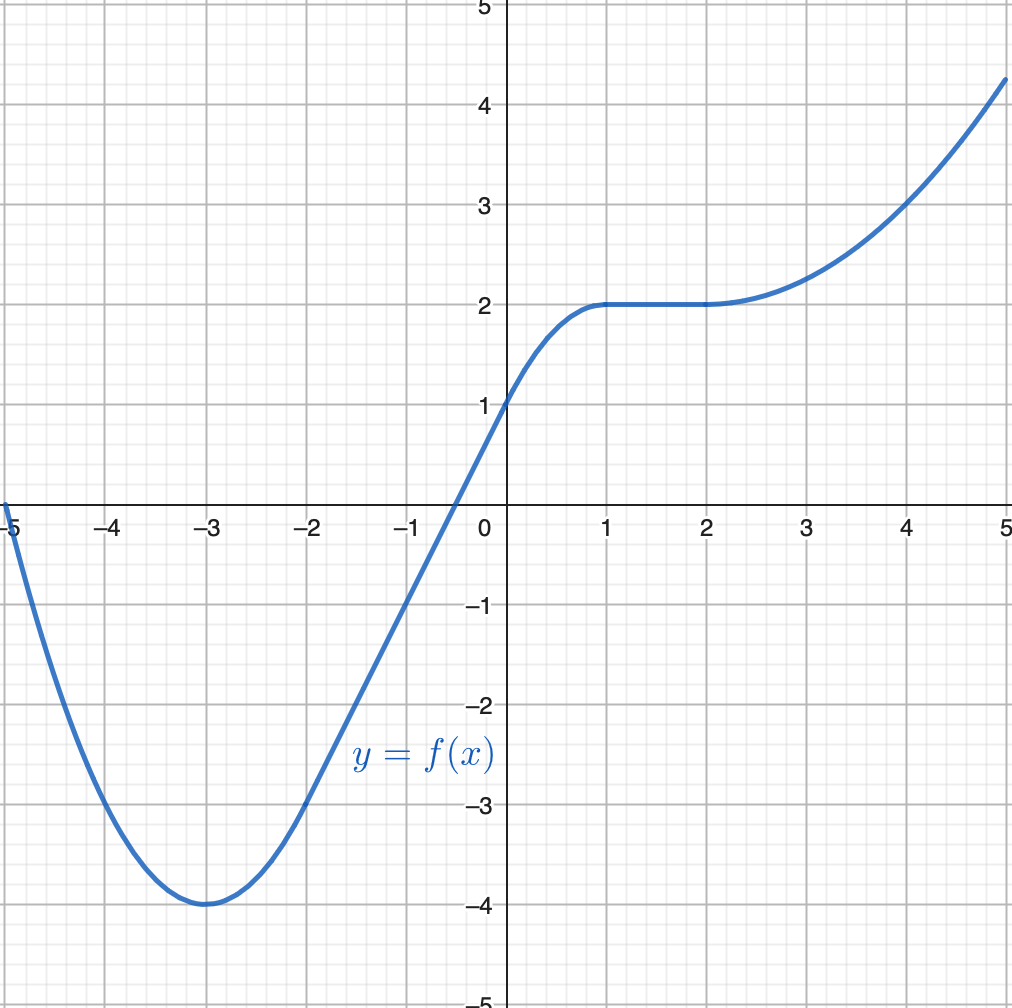
\includegraphics{images/CP-1-LT-1-graph-F23.png}} \hspace{0.25in} \scalebox{0.4}{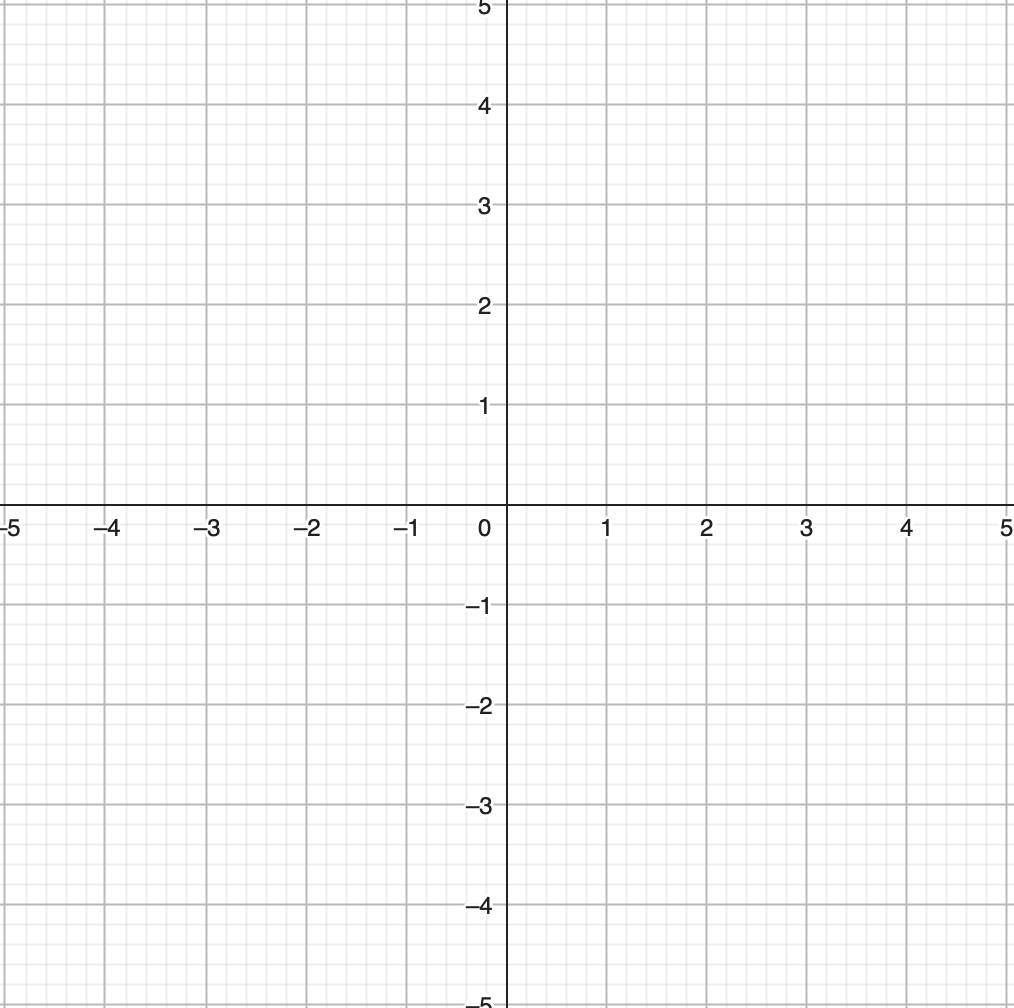
\includegraphics{images/CP-1-LT-1-grid-F23.png}} \\
\end{center}

		\item Consider the two piecewise linear functions $p$ and $q$ given by the figure below.


Determine each of the following derivative values that involve functions that are defined in terms of $p$ and $q$.  Clearly show your work and thinking using proper notation. (If I were you, I'd write out formulas for $m'(x)$ and $p'(x)$ before plugging in numbers.) 

\begin{center}
\scalebox{0.4}{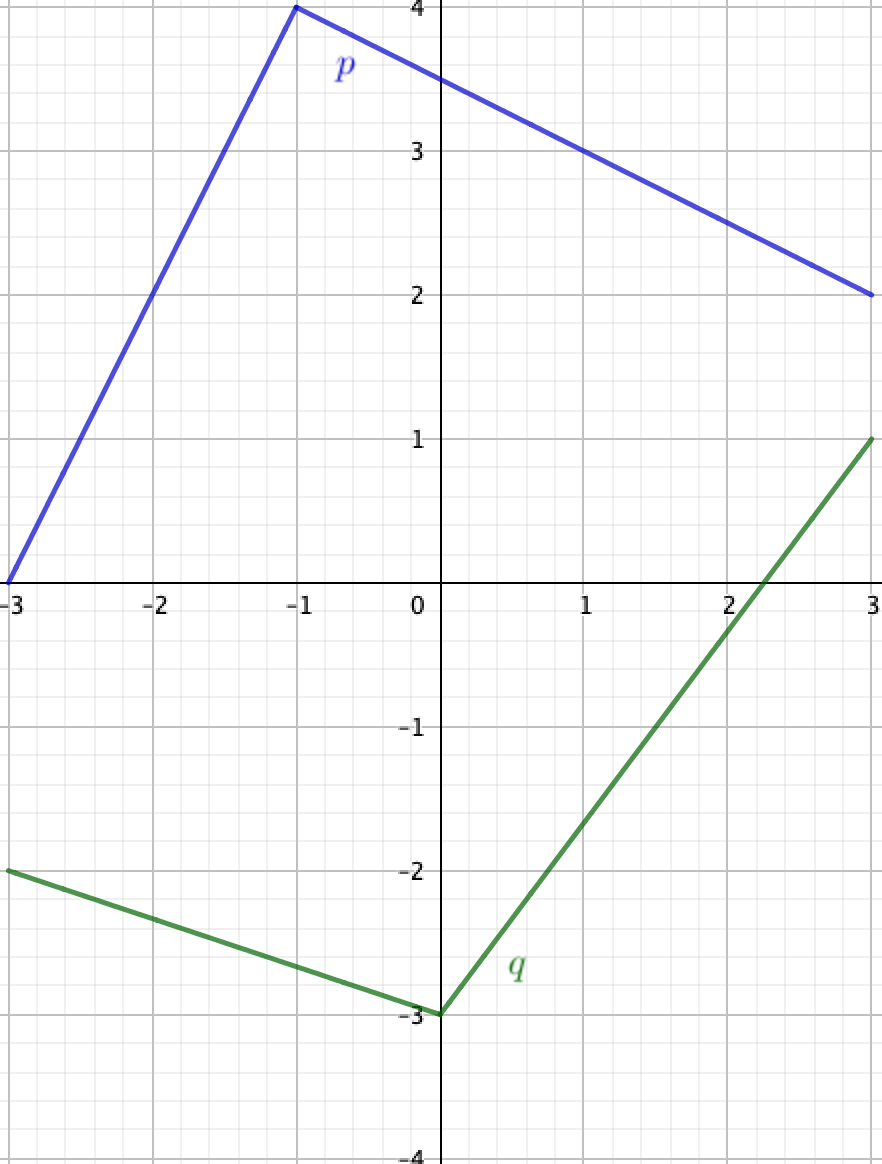
\includegraphics{images/CP7-11-3LTs.png}} \hspace{0.25in} \scalebox{0.5}{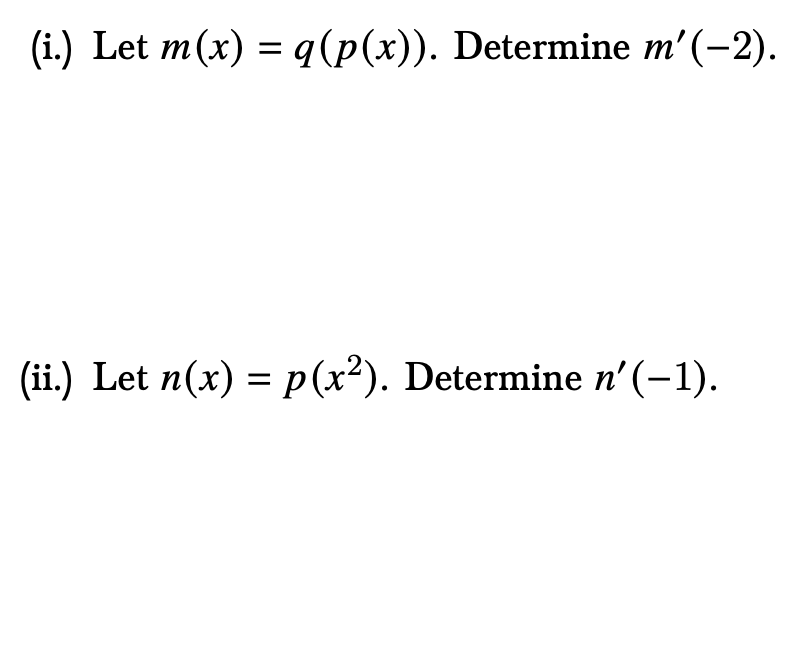
\includegraphics{images/CP-1-side-by-side-F23.png}} 
\end{center}

\vfill

Turn page over now please :)

\pagebreak

\item Consider $\displaystyle \int \dfrac{1}{x} \, dx$.

\begin{enumerate}[(a)]
    \item What does this mean, in human words?
    \vfill
    \item The antiderivative power rule won't work for this function. Why not? What goes wrong?
    \vfill
    \item What's the actual answer to this question? (This is not a trick question. There \textit{is} a good answer; it's not ``undefined'' or anything like that.)
    \vfill
    \item Write some human words explaining why your answer is right.
    \vfill
\end{enumerate}


\item Evaluate the following definite integral exactly using the Fundamental Theorem of Calculus.  Show your full work and thinking using proper notation.

$\displaystyle \int_1^3 \left(4x^2 + \frac{1}{x^2} - \frac{2}{x} \right) \, dx$
\vfill
\end{enumerate}
\end{document}